\documentclass[14pt]{beamer}


\usepackage{color}
\usepackage{tikz}


\mode<presentation>
{
\usetheme{AlpesLasers}
\setbeamercovered{transparent}
  %\setbeamertemplate{footline}[frame number] 
  %\setbeamertemplate{navigation symbols}{ 
  %\hskip 0.3cm
  %\insertframenumber / \inserttotalframenumber  % <<< frame #
  %\insertpagenumber / \insertpresentationendpage % <<< page #
%} 
}

% font definitions, try \usepackage{ae} instead of the following
% three lines if you don't like this look
\usepackage{listings}
\lstloadlanguages{python}

\usepackage{mathptmx}
\usepackage[scaled=.90]{helvet}
\usepackage{courier}
\usepackage[T1]{fontenc}
\usepackage[english]{babel}
\usepackage[latin1]{inputenc}
\title{Designing an efficient simulation framework}
%\subtitle{A little overview}
\author{St\'ephane Poss}
\date{\today}
% This is only inserted into the PDF information catalog. Can be left
% out.
\subject{PYTHON}

\lstdefinestyle{custompy}{
  belowcaptionskip=1\baselineskip,
  breaklines=true,
  xleftmargin=\parindent,
  language=python,
  showstringspaces=false,
  basicstyle=\footnotesize\ttfamily,
  keywordstyle=\bfseries\color{green!40!black},
  commentstyle=\itshape\color{purple!40!black},
  identifierstyle=\color{blue},
  stringstyle=\color{orange},
}
\lstdefinestyle{customsh}{
  belowcaptionskip=1\baselineskip,
  breaklines=true,
  xleftmargin=\parindent,
  language=bash,
  showstringspaces=false,
  basicstyle=\footnotesize\ttfamily,
  keywordstyle=\bfseries\color{green!40!black},
  commentstyle=\itshape\color{purple!40!black},
  identifierstyle=\color{blue},
  stringstyle=\color{orange},
}
\lstdefinestyle{customcpp}{
  belowcaptionskip=1\baselineskip,
  breaklines=true,
  xleftmargin=\parindent,
  language=C++,
  showstringspaces=false,
  basicstyle=\footnotesize\ttfamily,
  keywordstyle=\bfseries\color{green!40!black},
  commentstyle=\itshape\color{purple!40!black},
  identifierstyle=\color{blue},
  stringstyle=\color{orange},
}

\begin{document}
\begin{frame}[plain]
\titlepage
\end{frame}

\begin{frame}
\tableofcontents
\end{frame}

\section{Motivation}
\begin{frame}
\frametitle{Why this training?}

\includegraphics[width=\textwidth]{comp_prog_works_but_dangerous}
\end{frame}
\note{This training is designed to show you the issues faced by (mostly) students during their PhD when it comes to using computers to do part of the work. As the illustrations shows, it's a 'normal' situation. I do not know anybody that did not have this case at least once.}

\begin{frame}
\centering

\includegraphics[width=0.7\textwidth]{disclaimer}

\end{frame}
\note{The following presentation is the results of years of troubles, 3 work places with different practices, and discussions with friends/colleagues. It may not represent the complete situation, and some of the topics mentioned here can be already known by some people. I tried to collect the worst practices and the best ideas to fix them, and I may have missed some things.}

\begin{frame}
Ch. Hugon, INFN fellow:
\begin{quote}
Maybe it's not worth telling people about this stuff, maybe it's worth for them to discover the do's and don'ts by themselves...
\end{quote}
\end{frame}
\note{This quote from a friend of mine, former colleague and student is representative of the current state of affairs: it's hard to teach this stuff, and showing things may not be enough, you'd need to experience them to feel the pain. Nevertheless, maybe this talk will give you tools to face the problems in a sane manner.}

\section{Definitions}
\begin{frame}
Definitions
\end{frame}

\begin{frame}
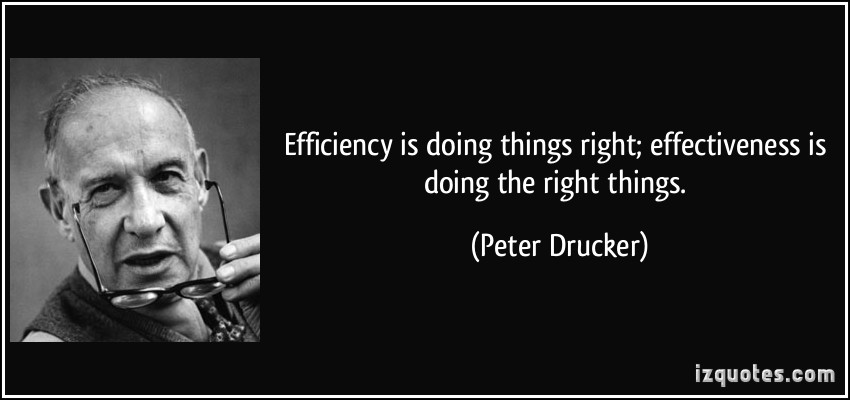
\includegraphics[width=\textwidth]{quote-efficiency-is-doing-things-right-effectiveness-is-doing-the-right-things-peter-drucker-53210}
\end{frame}
\note{Efficiency and effectiveness are complementary. I will concentrate on the first, as it's not my role to tell what you should do. I will tell you how though.}


\begin{frame}
Simulation framework
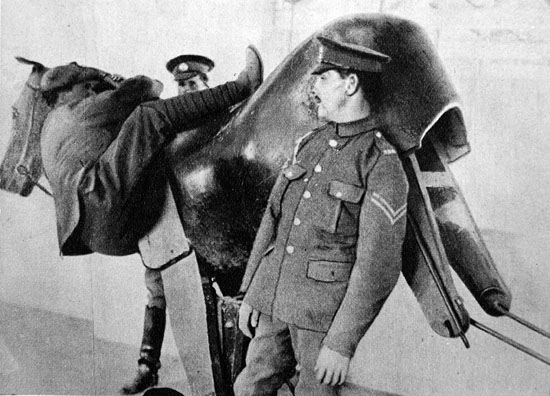
\includegraphics[width=\textwidth]{Horse_simulator_WWI}
\end{frame}
\note{Defining simulation framework goes to defining modeling. Wikipedia has a nice article on this, where the image is taken from. It's a horse simulator used during WW1. It's important to define properly what we mean by simulation as it drives the rest of the talk.}

\begin{frame}
\frametitle{Why simulations?}
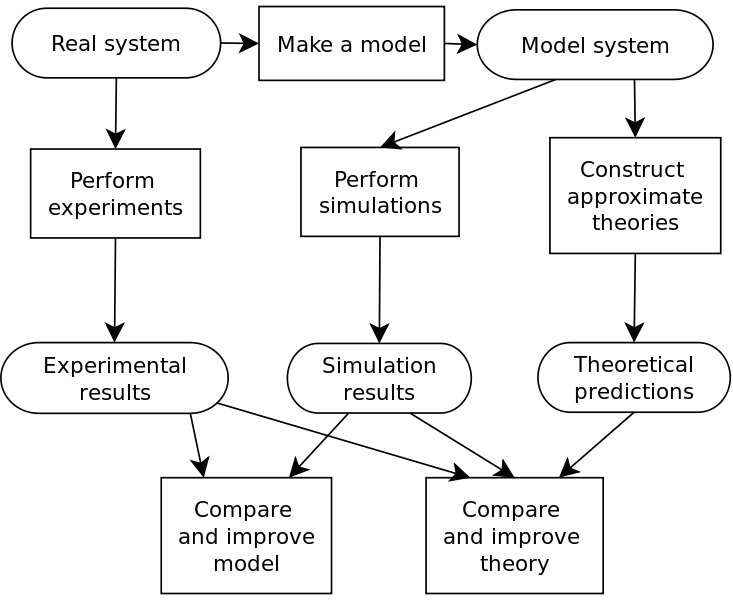
\includegraphics[width=\textwidth]{733px-Molecular_simulation_process}
\end{frame}
\note{Starting from a real life situation, we want to put a theory on it, because we want to predict the future behavior of the system. If there is a theory, there is a model. The model may not be a complete representation of the theory. This, the simulation has 2 purposes: improve the model when comparing with experiment, or improve the theory by numerically checking its soundness.}

\begin{frame}
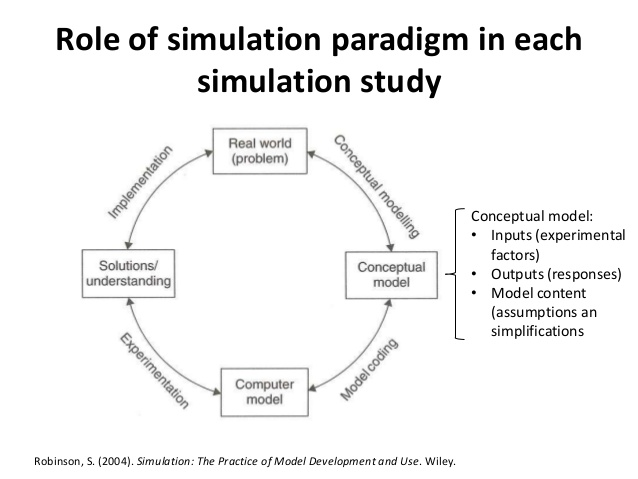
\includegraphics[width=1.1\textwidth]{agentbased-modeling-system-dynamics-or-discreteevent-simulation-modeling-paradigm-for-supply-chains-simulation-3-638}
\end{frame}
\note{This shows more or less the same ideas as previously}


\section{The usual situation}
\begin{frame}
\frametitle{The usual situation}

\includegraphics[width=\textwidth]{painful_but_true}
\end{frame}
\note{I will now tell you a bit about how things are usually done during a PhD (and beyond). It's a bit ugly and some of you may laugh due to experience.}
\begin{frame}
\frametitle{1st year PhD}
\begin{itemize}
\item Create files on the fly, in the same directory
\item Overwrite code, changes drastically every day, DRY principle NOT applied
\item Code monolithic as much as possible, data structure unclear
\item Output are named test\_1, test\_2, test\_1\_altered, lum\_check\_260815, plots are all in the same directory
\end{itemize}
\end{frame}
\note{
A big mess!
}

\begin{frame}
\frametitle{1st year PhD}
\begin{itemize}
\item Application version does not matter, hacked to fit need if possible.
\item Data stored only on personal drive, not backed up
\item Sharing of code/data via email, but unusable
\item All analysis are slightly different, can hardly be shared between run points
\end{itemize}
\end{frame}

\begin{frame}
\frametitle{2nd year PhD}
\begin{itemize}
\item Use directory structure\\ /data/thesis/simu/260815/p1/p2/file\_p1\_p2.out, input.txt, source code
\item Code organized by date: changes imply copy of the code structure
\item Code structured: reused functions appear
\item Application version is checked regularly, new features asked to dev being added on demand (if possible)
\end{itemize}
\end{frame}
\note{\begin{itemize}
\item How to add info in fixed path? variable and rigid
\item How do you know which code contains which change?
\end{itemize}
}
\begin{frame}
\frametitle{2nd year PhD}
\begin{itemize}
\item Log book used
\item Data shared via NFS/FTP/SCP/etc. 
\item Code base clearer 
\item Recipes to process data in place, still done manually
\end{itemize}
\end{frame}
\note{
\begin{itemize}
\item Log book stores links between data and source/inputs
\item training takes a few days
\item API changes not backward compatible
\end{itemize}
}

\begin{frame}
\frametitle{3rd year PhD}
\begin{itemize}
\item Meta description of data
\item Files stored on persistent drive
\item Synergy with application developer
\item Core applications wrapped to read/store I/O directly in DB
\item Code properly documented, API well defined and stable
\end{itemize}
\end{frame}
\note{
\begin{itemize}
\item flexible, extensible, easy to find what you want
\item Use relational databases
\item setup backup procedures: backup, distributed, shared
\item Interactions between data storage and processing simplified
\end{itemize}
}

\begin{frame}
\frametitle{3rd year PhD}
\begin{itemize}
\item Code structured properly
\item Code versioning used extensively
\item Automatic processing of data
\item Use code from elsewhere
\end{itemize}
\end{frame}
\note{
\begin{itemize}
\item Code is organized in logical elements, core libraries stand out and reused. data structures are decoupled from functions
\item SVN/GIT
\item workflows, data driven processing
\item Don't reinvent the wheel
\end{itemize}
}

\section{Where we go from there}
\begin{frame}
\centering
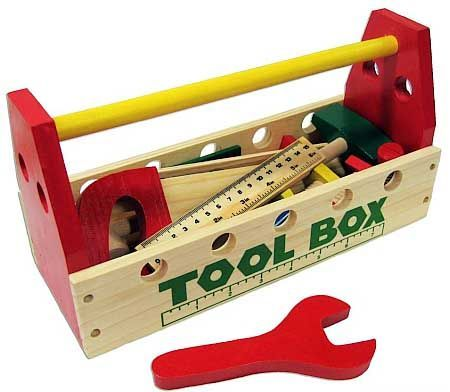
\includegraphics[width=0.8\textwidth]{wooden_tool_box}

\end{frame}

\subsection{Coding practices}
\begin{frame}
\frametitle{Version control}
\centering
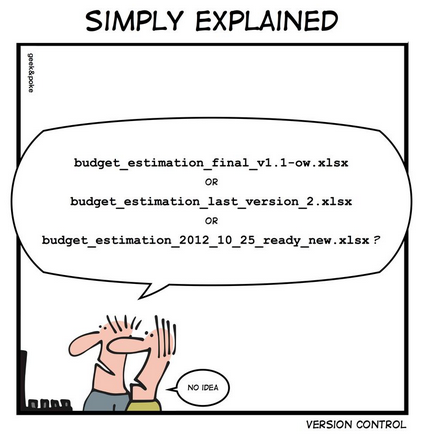
\includegraphics[width=0.8\textwidth]{Version-Control-Comic}

\end{frame}

\begin{frame}
\frametitle{Version control}
\begin{block}{How?}
\begin{itemize}
\item[SVN] Centralized: need to get all changes from master server every time
\item[\alert{Git}] Distributed: all history local, can have many parallel copies
\end{itemize}

\includegraphics[width=0.5\textwidth]{svn-name-banner.jpg}$\quad$

\includegraphics[width=0.3\textwidth]{Git-Logo-2Color.png}
\end{block}
\end{frame}


\begin{frame}
\frametitle{Documentation}
\centering

\includegraphics[width=\textwidth]{docu}

\end{frame}
\note{
Documentation is fundamental! People tend to overlook it, because they don't see the point. They don't see that maybe, someday, someone will reuse their stuff. Or they think that no one cares. It's wrong!
}

\begin{frame}
\frametitle{Documentation}
\centering
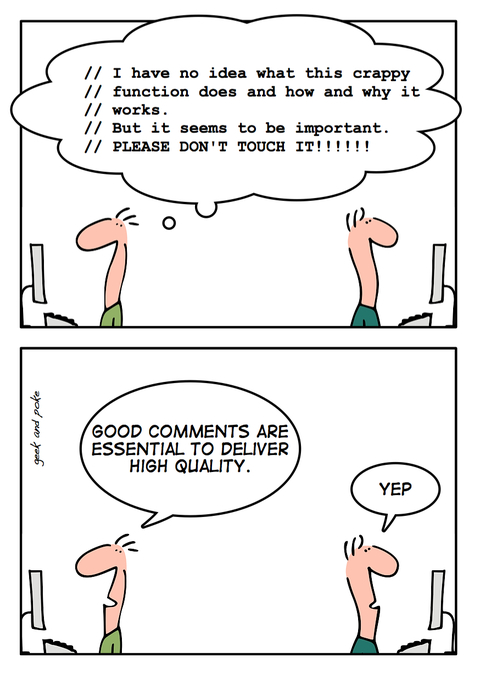
\includegraphics[width=0.6\textwidth]{goodcomments}

\end{frame}
\note{Example of bad doc!}

\begin{frame}
\frametitle{Documentation}
\begin{itemize}
\item Code documentation isn't enough
\item Tests (if any) aren't enough
\item Think documentation as teaching
\end{itemize}
\end{frame}
\note{ 
Remember there is someone that will be using your stuff after you left!

Tests should exist!
}

\begin{frame}
\frametitle{Coding practices}
\centering

\includegraphics[width=\textwidth]{dontrepeatyourself_motivator_2}

\end{frame}

\subsection{PYTHON}
\begin{frame}
\frametitle{Python}
Perfect scripting language for the physicist!
\end{frame}
\note{Been using Python for many years. Prefer it to C++. Easy to learn and use. Lack of compilation saves many headaches.}


\begin{frame}
\frametitle{Python}
\begin{itemize}
\item C/C++: effective language, not efficient in its use, but efficient in CPU usage\\~
\item Python: effective and efficient language for the physicist, not as efficient in CPU cycles
\end{itemize}
\end{frame}
\note{Use the right language for a given purpose!}

\begin{frame}
\frametitle{Must-use libraries}
\begin{itemize}
\item numpy: matlab like interface to data
\item scipy: machine learning tools
\item pandas: data analysis
\item sympy: symbolic computations
\item matplotlib: plots
\item sqlalchemy: DB overlay
\end{itemize}
Many other utilities available!
\end{frame}

\begin{frame}
\centering
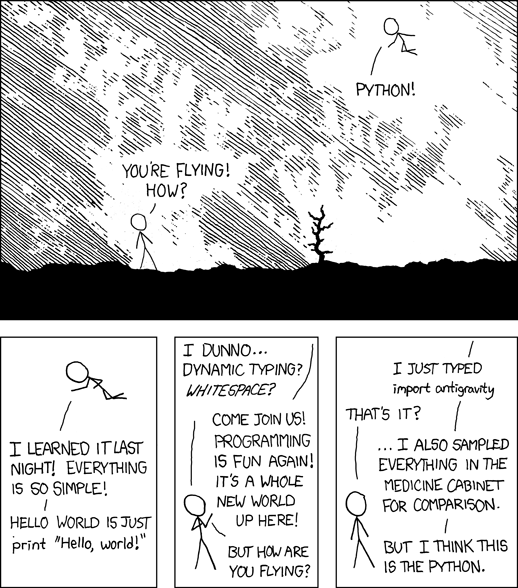
\includegraphics[width=0.7\textwidth]{python}

\end{frame}

\subsection{Application control}
\begin{frame}
\frametitle{Control your applications}
\begin{itemize}
\item Control: keep track of your inputs and outputs
\end{itemize}
\end{frame}

\subsection{Data storage}
\begin{frame}
\frametitle{Data storage and metadata}
\end{frame}

\begin{frame}
\frametitle{Data base systems}
\end{frame}

\begin{frame}
\frametitle{iRods}
\end{frame}

\begin{frame}
\frametitle{Sumatra}
\end{frame}

\section{Real life example}
\begin{frame}
\frametitle{Real life example: Alpes Lasers simulation framework}
\end{frame}

\section{Conclusions}
\begin{frame}

\includegraphics[width=\textwidth]{sad_truth}
\end{frame}

\end{document}